%%%%%%%%%%%%%%%%%%%%%%%%%%%%%%%%%%%%%%%%%%%%%%%%%%%%%%%%%%%%%%%%%%%%%%
% LaTeX Example: Project Report
%
% Source: http://www.howtotex.com
%%%%%%%%%%%%%%%%%%%%%%%%%%%%%%%%%%%%%%%%%%%%%%%%%%%%%%%%%%%%%%%%%%%%%%

%%% Preamble
\documentclass[paper=a4, fontsize=11pt]{scrartcl}
\usepackage[T1]{fontenc}
\usepackage{fourier}

\usepackage{cite}
\usepackage{listings,xcolor}
\usepackage{url}
\usepackage{hyperref}
\usepackage[english]{babel}	% English language/hyphenation
\usepackage[protrusion=true,expansion=true]{microtype}
\usepackage{amsmath,amsfonts,amsthm} % Math packages
\usepackage[pdftex]{graphicx}
\usepackage{url}

\usepackage{graphicx}
\graphicspath{ {images/} }

%%% Custom sectioning
\usepackage{sectsty}
\allsectionsfont{\centering \normalfont\scshape}


%%% Custom headers/footers (fancyhdr package)
\usepackage{fancyhdr}
\pagestyle{fancyplain}
\fancyhead{}                       % No page header
\fancyfoot[L]{}                    % Empty
\fancyfoot[C]{}                    % Empty
\fancyfoot[R]{\thepage}            % Pagenumbering
\renewcommand{\headrulewidth}{0pt} % Remove header underlines
\renewcommand{\footrulewidth}{0pt} % Remove footer underlines
\setlength{\headheight}{13.6pt}


%%% Equation and float numbering
\numberwithin{equation}{section} % Equationnumbering: section.eq#
\numberwithin{figure}{section}   % Figurenumbering: section.fig#
\numberwithin{table}{section}    % Tablenumbering: section.tab#


%%% Maketitle metadata
\newcommand{\horrule}[1]{\rule{\linewidth}{#1}} % Horizontal rule

\title{
  \usefont{OT1}{bch}{b}{n}
  \normalfont \normalsize \textsc{Alliander} \\ [25pt]
  \horrule{0.5pt} \\[0.4cm]
  \huge Decentralized authorization of access to energy data \\
  \horrule{2pt} \\[0.5cm]
}
\author{
\normalfont \normalsize
Erwin Rooijakkers\\[-3pt] \normalsize
\today
}
\date{}

%%% Begin document
\begin{document}
\maketitle

\section{Introduction}

% Perhaps name some applications of blockchain technology. And Alliander's
% Joulliette project.

Within Alliander various projects (like Tippiq, HelloData, and GateKeeper) work
on the use case of authorizing the access of energy data for P1-device to app,
so that the consumer is in control over his data. Because of the characteristics
of the blockchain (immutability, decentralization, independence, automatic
settlement, availability, reachability), it seems beneficial to decentralize the
authorization business logic on a public or private blockchain. In this document
a prototype for authorizing data access on the Ethereum blockchain is
introduced, and future recommendations are provided.\\

The Ethereum blockchain is an immutable, distributed ledger with a virtual
machine \cite{ethereum}. Using peer-to-peer technology, cryptography, and
consensus formation algorithms, no trusted third party is necessary to keep an
"official" copy of the state of the Ethereum Virtual Machine (EVM). Code in
so-called "smart contracts" can be executed and publicly verified. To change the
state of the blockchain fees have to be paid in the cryptocurrency (Ether).
Querying the Ethereum blockchain is free and can be done by anyone with access
to the ledger.\\

\begin{figure}[h]
  \centering
  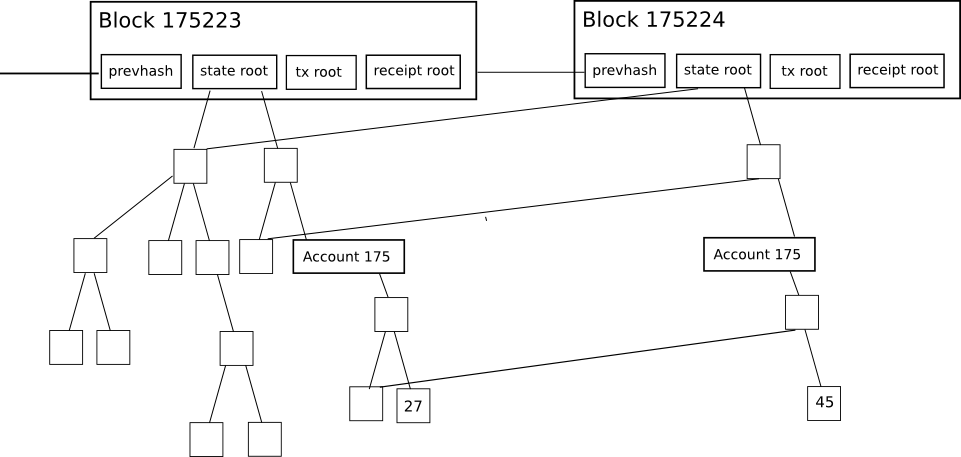
\includegraphics[width=\textwidth]{ethblockchain_full}
  \caption{Ethereum blockchain stores three kinds of information: transactions, receipts, state.}
  \label{fig:ethblockchain_full}
\end{figure}

In Figure \ref{fig:ethblockchain_full} obtained from ~\cite{ethereum} based on
~\cite{bitcoin} the Ethereum blockchain is visualized. The Ethereum blockchain
is a ``chain'' of ``blocks'' that is shared over every full node in the network.
Each block consists of a hash of the previous block, transactions (transferring
the cryptocurrency Ether from one address to another), receipts (state changes)
and state (the state of the EVM). Because the Ethereum blockchain contains state
alongside transactions, on the EVM a Turing complete programming language is
available that enables smart contracts \cite{ethereum}.\\

To reach consensus on the state of the ``real'' blockchain (to guard against
``double spending'' attacks where an attacker makes a longer official chain)
various algorithms can be used; the most famous ones being Proof of Work (PoW)
and Proof of Stake (PoS). In PoW consensus is reached by the solution of a
cryptographic puzzle over the state and transactions, that takes computer power
to solve. Because it takes so much computer power to find a solution, the
network can trust that the result was reached by consensus (it would take an
attacker at least 51\% of computer power to built a longer chain). In PoS trust
is reached because people who are invested in the network set aside their
cryptocurrency to stake for receipts and transactions. Ethereum currently works
with PoW, but will switch to PoS sometime this year \cite{ethereum}.\\

Now, authorizing energy data on the Ethereum blockchain, and its benefits and
limitations, will be discussed.\\

\section{Authorizing energy data on the blockchain}

There are three entities at play when authorizing access to energy data:

\begin{enumerate}
  \item Device (IoT-device that provides energy data)
  \item Consumer (owner of an IoT-device)
  \item App (service provider that wants to do something with energy data)
\end{enumerate}

The consumer, app, and device need to have an address on the Ethereum blockchain
(key pair). Because of the properties of blockchain addresses it can be ensured
that the actions are executed by the entities involved. A device can be claimed
by a consumer. And a consumer can then give access to the app. Finally,
a device can check if an app has access.\\

A smart contract that implements this logic is shown below in \ref{prototype} Prototype.\\

\section{Prototype}
\label{prototype}

% CODE
\lstset{%
basicstyle=\scriptsize\ttfamily,numbersep=5mm, numbers=left, numberstyle=\tiny,
language=java,
breaklines=true,
%frame=single,
framexleftmargin=8mm, xleftmargin=8mm,
prebreak = \raisebox{0ex}[0ex][0ex]{\ensuremath{\hookleftarrow}},
%backgroundcolor=\color{green!5},
frameround=fttt,escapeinside=??,
%rulecolor=\color{red},
morekeywords={function,address,require,contract,constant,returns,bool,mapping,is,return,import,pragma},
keywordstyle=\color[rgb]{0,0,1},                    % keywords
commentstyle=\color[rgb]{0.133,0.545,0.133},    % comments
stringstyle=\color[rgb]{0.627,0.126,0.941}  % strings
%columns=fullflexible
}%
\lstinputlisting{SmartEnergyAuthorizations.sol}

The above smart contract is deployed on the Ethereum test net. It is possible to
interact with this smart contract back-end via the front-end deployed on
\url{http://erooijak.simple-webhosting.eu}.\\

\section{Discussion}
\label{discussion}

There are some limitations to authorizing access to energy data on the Ethereum
blockchain and in the smart contract above. These are stated below as problem,
and underneath every problem a possible solution is provided.

\begin{itemize}
\item \textbf{Problem:} Performing the transactions (e.g., claiming a device)
  costs money (fees on Ethereum blockchain). This means that the consumer and
  device have to pay. \\\textbf{Solution:} The IOTA Tangle blockchain does not
  have this limitation \cite{iota}. It can, in the future, also share energy
  data between IoT-devices in an end-to-end encrypted manner \cite{iotamam} (!).
\item \textbf{Problem:} Scalability of the blockchain. When more devices start
  using the Ethereum blockchain state changes and transactions might not be
  included in blocks. This can lead to increased transaction fees or longer
  during transactions. \\\textbf{Solution:} The IOTA Tangle \cite{iota} is a
  ``blockchainless blockchain'' where consensus formation is not separated from
  the performing of transactions (every previous transaction needs to validate
  two earlier transactions). This is why the IOTA Tangle has no scalability
  issues. It would solve this problem. (Note: IOTA Tangle does not yet implement
  smart contracts because timestamps are difficult to implement, so another way
  to do authorization needs to be found, or wait till the problem is solved,
  which it is almost, e.g., \cite{iotatimestamps}).
\item \textbf{Problem:} Scalability of implementation. If a lot of devices and
  authorizations are stored in the smart contract it might lead to performance
  problems when it stores many devices and authorizations. \\\textbf{Solution:}
  Use an appropriate data structure; or use offchain or off-Tangle processing.
\item \textbf{Problem:} In the current smart contract, when a device changes
  ownership the old authorizations are taken along to the new consumer. The
  reason is that a mapping type does not know which keys it contains.
  \\\textbf{Solution:} To fix this another data structure needs to be used, that
  can be iterated over and cleaned when switching ownership. For example an
  IterableMapping.
\item \textbf{Problem:} In the current smart contract, the list of devices for a
  consumer are not iterable. To provide a convenient user interface around the
  smart contract back-end this type of information needs to be queryable. But
  maybe such a UI is not a requirement. \\\textbf{Solution:} Same as above.
\item \textbf{Problem:} A consumer cannot provide a granularity of access to a
  device (e.g., only part of the data of a device, like only realtime data but
  not the history). \\\textbf{Solution:} To fix this other data structures need
  to be used in the contract, like the IterableMapping mentioned above. Wherein
  also the capabilities of the device can be stored.
\item \textbf{Problem:} Authorization data is publicly available and
  inspectable. \\\textbf{Solution:} This can be solved by a proper anonymous
  identity management system like IRMA \cite{irma} or Sovrin \cite{sovrin},
  where only the attributes of an identity that are necessary (e.g., does a
  consumer live on the address of the device?) are available, in a
  non-identifiable manner.
\end{itemize}

\section{Conclusion}

Authorizing access to energy data on the Ethereum blockchain is doable. It makes
all the benefits of the blockchain automatically available. The authorization
data information cannot be tempered with, it provides an immutable audit trail
of events, and it is convenient for a device to access the necessary
authorization information, or even for an app to access the data of a device,
even when the device is behind a firewall.\\

There are some limitations to using a blockchain for authorizing access to
energy data. Limitations coming from high transaction costs, the data structures
used in the contract, and identity management. A combination of IOTA Tangle, new
data structures, and an identity management system (like IRMA \cite{irma} or
Sovrin \cite{sovrin}) will help solve this.\\

I am convinced of the benefits of blockchain technology for authorizing (and
transporting) energy data and hope that we will build a data authorization
gateway backed by blockchain technology. \\

\bibliographystyle{unsrt}
\bibliography{references}

\end{document}
